\documentclass[sigconf]{acmart}

\AtBeginDocument{%
  \providecommand\BibTeX{{%
    \BibTeX}}}

\usepackage{graphicx}
\usepackage{hyperref}
\usepackage{float}

\begin{document}

\title{Social Media Data Science Pipelines Project Report: Dataset Measurements and Analysis}

\author{Devang Jagdale}
\email{djagdale@binghamton.edu}
\affiliation{% 
  \institution{Binghamton University}
  \city{Binghamton}
  \state{New York}
  \country{USA}}

\author{Tejas Hiremath}
\email{thiremath@binghamton.edu}
\affiliation{% 
  \institution{Binghamton University}
  \city{Binghamton}
  \state{New York}
  \country{USA}}

\author{Chaitanya Jha}
\email{cjha@binghamton.edu}
\affiliation{% 
  \institution{Binghamton University}
  \city{Binghamton}
  \state{New York}
  \country{USA}}

\maketitle

\section{Introduction}
This project builds on prior work to address key research questions about social media activity and sentiment analysis. We analyze temporal patterns, engagement metrics, and sentiment shifts across Reddit and 4chan data to answer our proposed research questions.

\section{Research Questions}
\begin{itemize}
    \item How do temporal patterns in social media activity correlate with engagement metrics like comments?
    \item How do shifts in sentiment metrics (e.g., happy, sad, angry, hopeful) correlate with key events and discussions in U.S. politics?
    \item How do tones and volumes of discussions differ between mentions of different political candidates or parties?
\end{itemize}

\section{Data and Methods}
Data was sourced from Reddit and 4chan datasets and processed using Python libraries such as Pandas and Plotly. The interactive tool built with Flask and Dash allowed querying and visualizing key analyses. Key analyses included:
\begin{itemize}
    \item Time-series analysis of activity and engagement.
    \item Sentiment analysis of user comments.
    \item Country-based analysis of comment distributions.
\end{itemize}

\subsection{Tools and Frameworks}
\begin{itemize}
    \item Flask/Dash for the interactive dashboard.
    \item Plotly for visualizations.
    \item Scikit-learn for sentiment analysis.
    \item PostgreSQL for dataset management.
\end{itemize}

\section{Web based Results and Discussion}

\subsection{Time-Series Analysis}
Figure1 shows combined activity from Reddit and 4chan. The analysis highlights peak activity hours and engagement patterns. In this graph we have added two filters where first is for date and second is for dataset selection.

\begin{figure}[H]
    \centering
    \begin{figure}
        \centering
        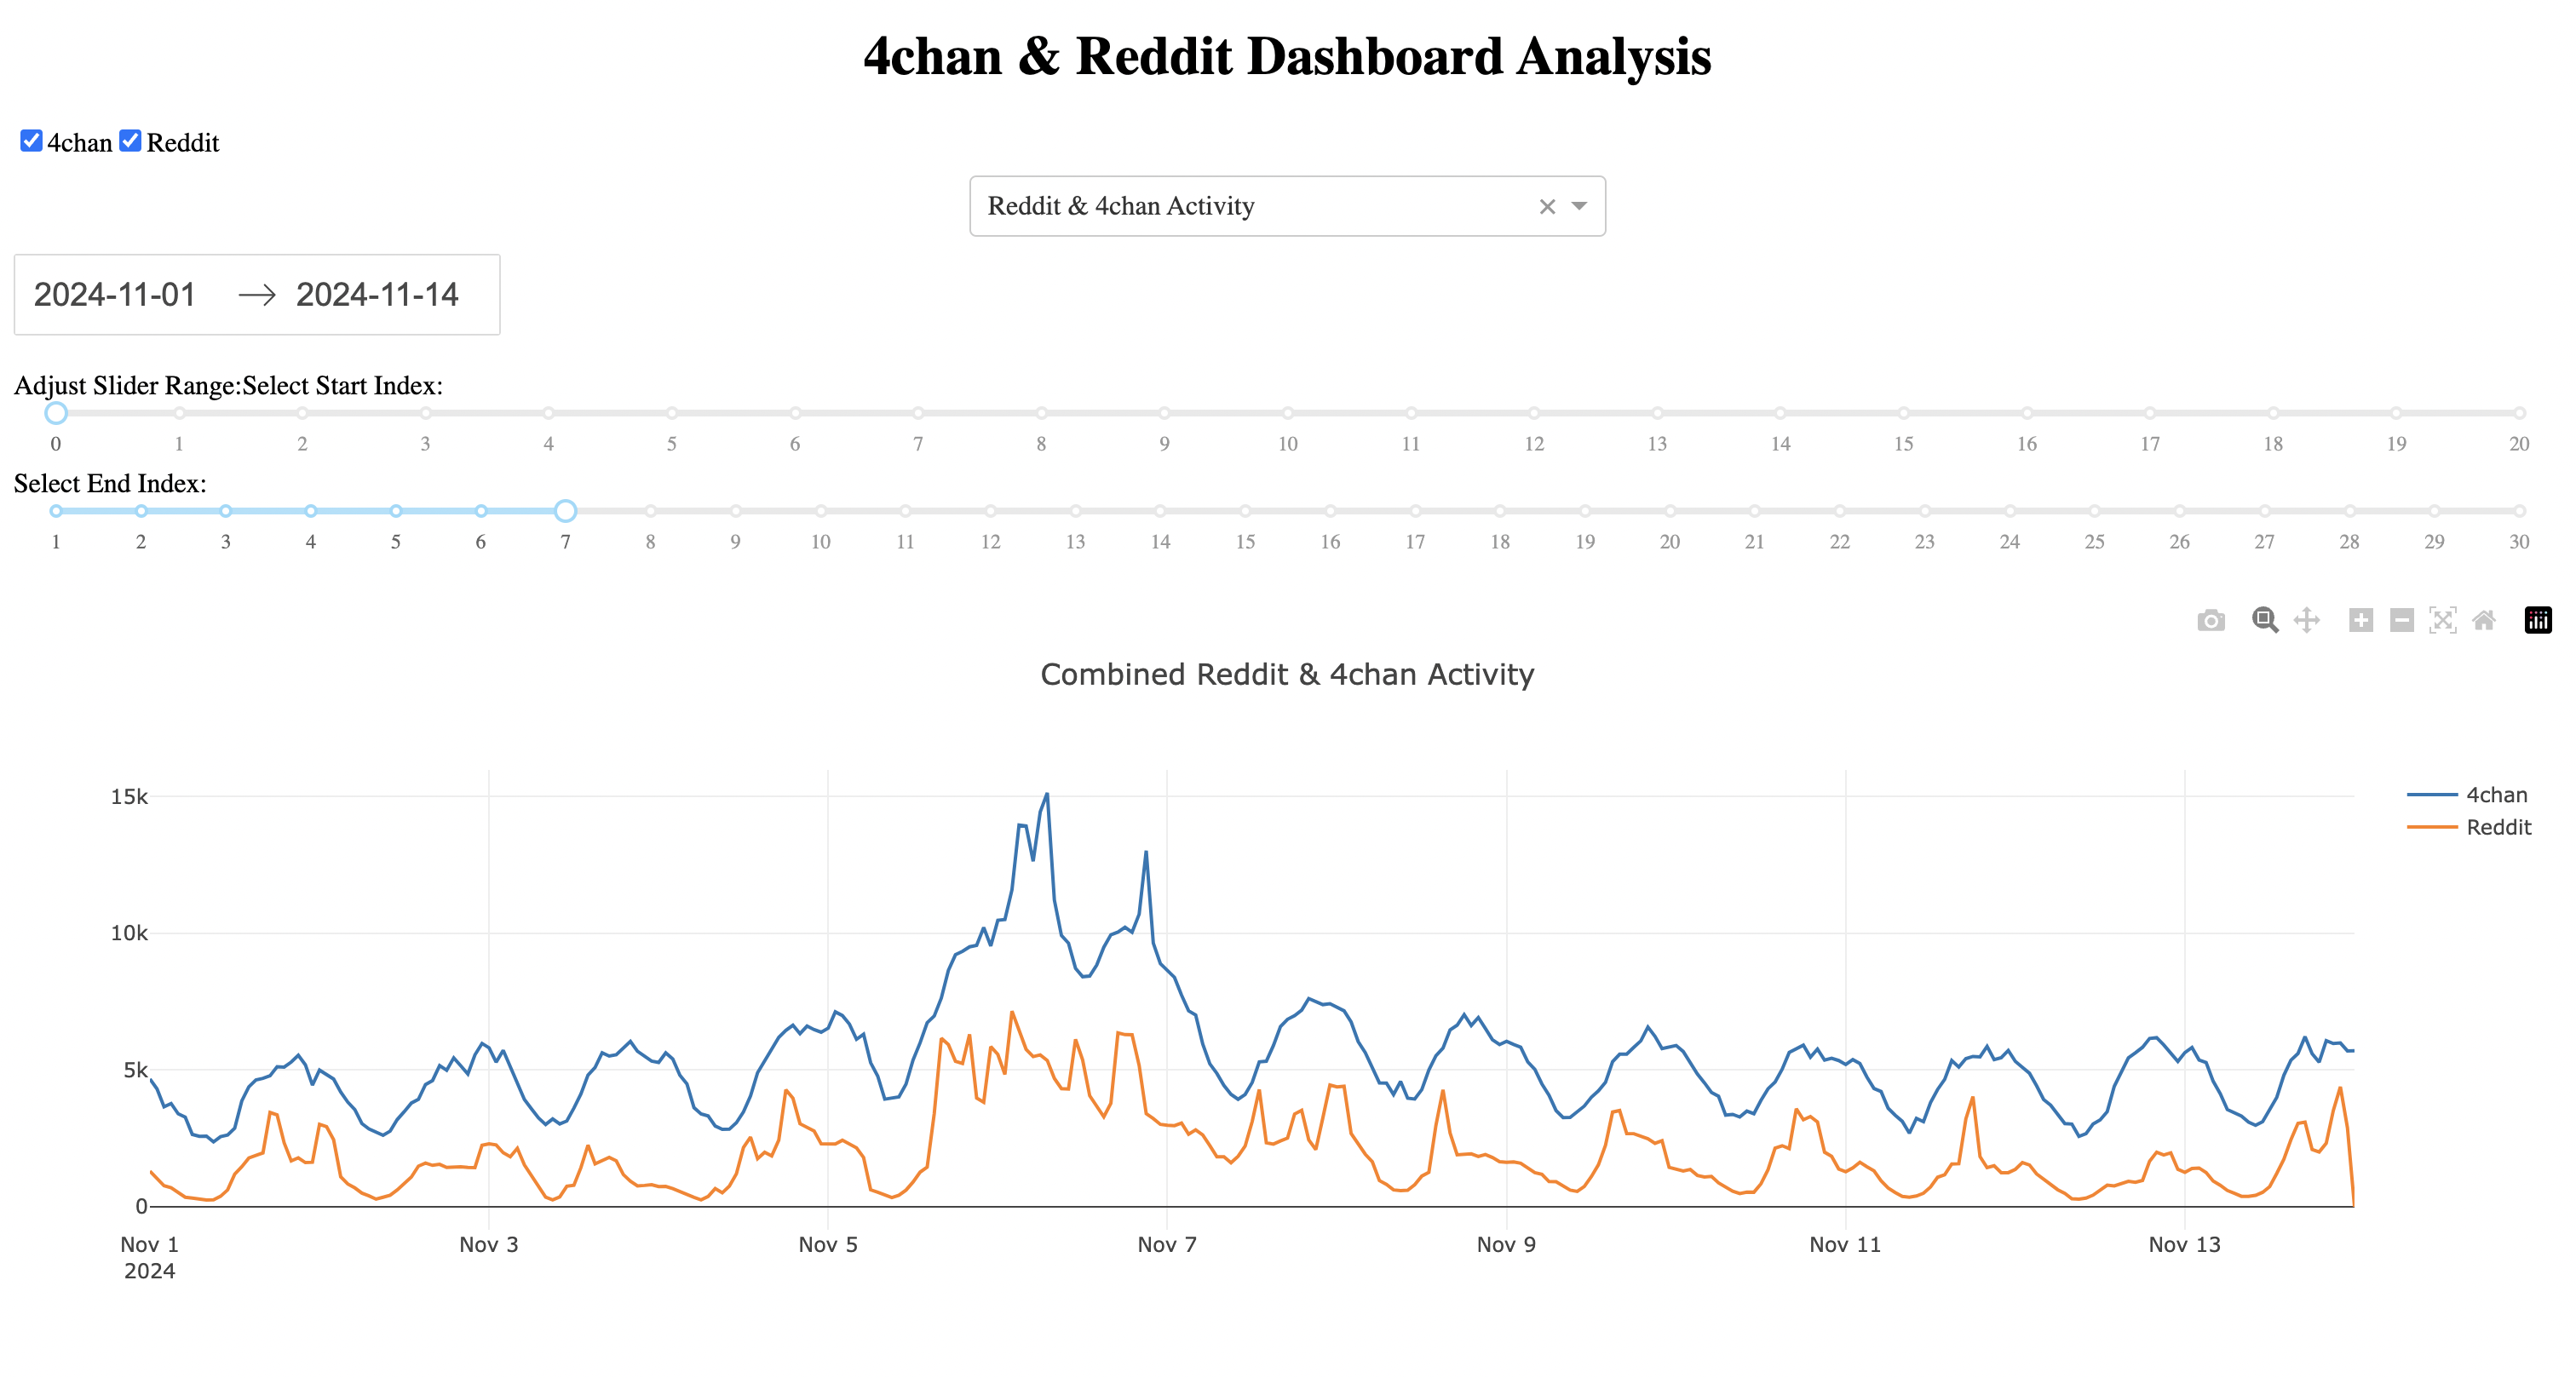
\includegraphics[width=0.5\linewidth]{image.png}
        \label{fig:enter-label}
    \end{figure}
    \caption{Time-series analysis of Reddit and 4chan activity.}
    \label{fig:time_series}
\end{figure}

\subsection{Sentiment Analysis}
Sentiment analysis revealed trends in user emotions during significant political events. Figure2 illustrates the sentiment breakdown across dates. Filters used were date and sentiment that you want to see across timeseries.

\begin{figure}[H]
    \centering
    \begin{figure}
        \centering
        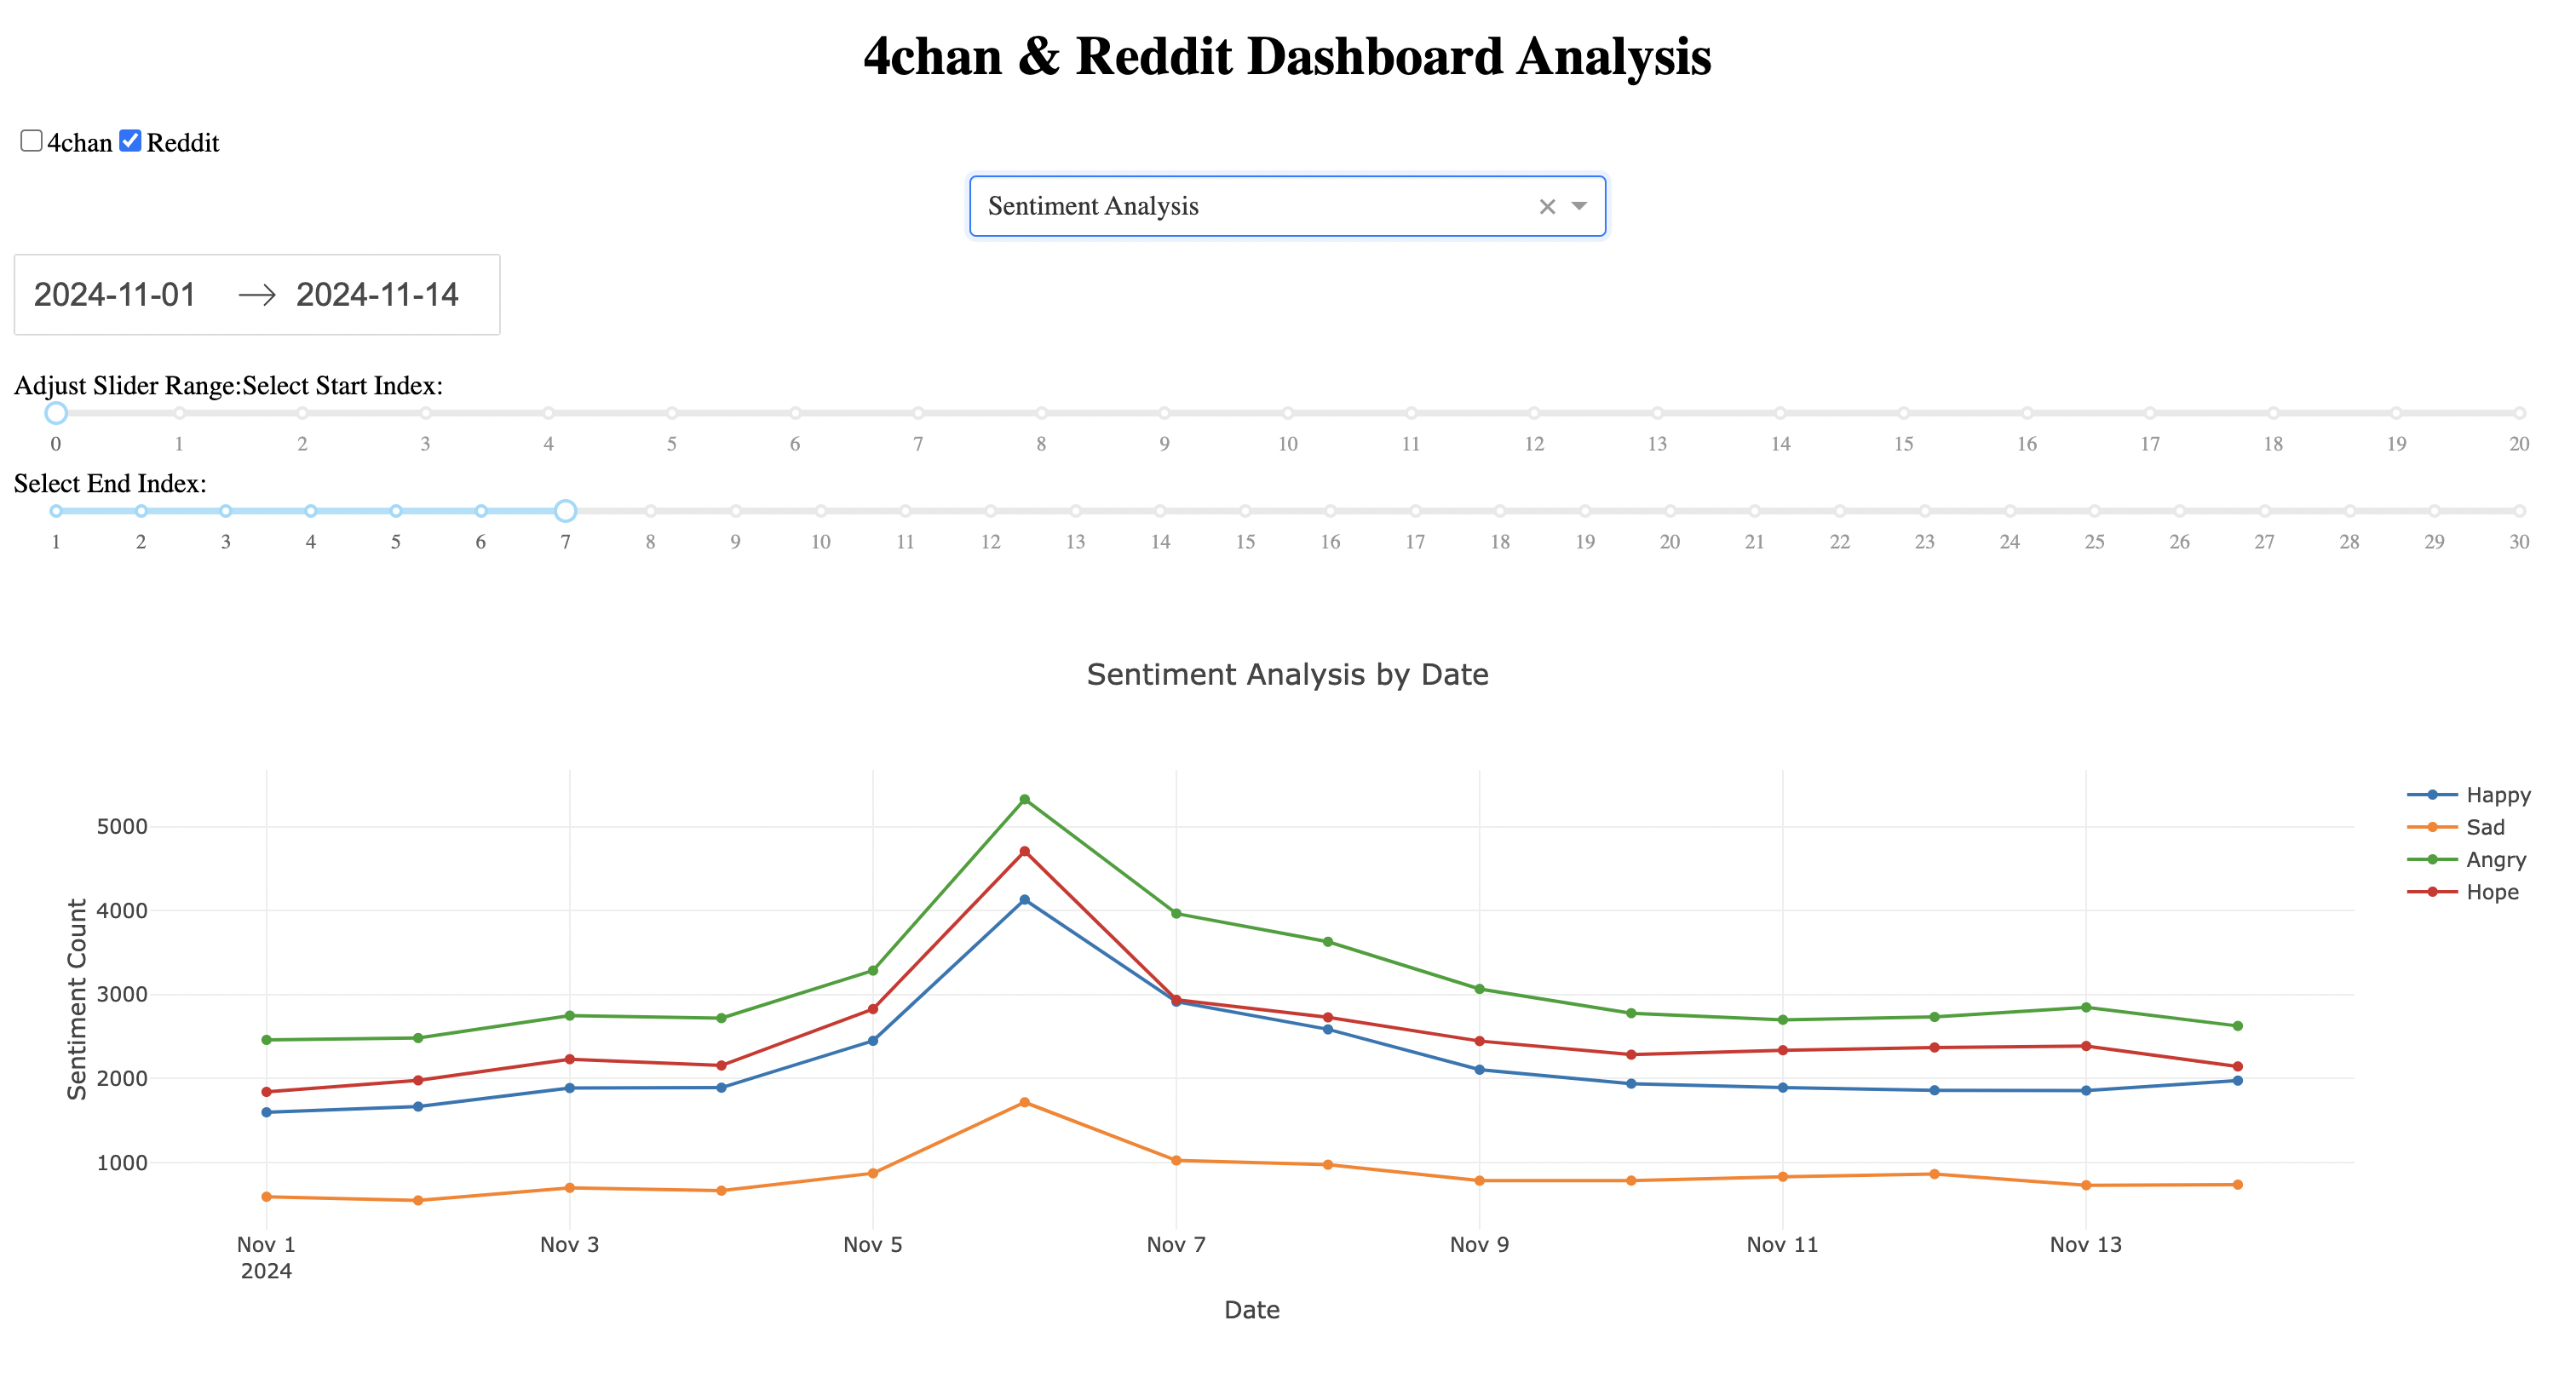
\includegraphics[width=0.5\linewidth]{image-3.png}
        \label{fig:enter-label}
    \end{figure}
    \caption{Sentiment analysis of Reddit and 4chan comments.}
    \label{fig:sentiment}
\end{figure}

\subsection{Country-Based Analysis}
Figure3 displays the distribution of comments by country, highlighting regions with high engagement. Filter created was of range of top countries like if I want to see countries ranging from top m to n ranking only.

\begin{figure}[H]
    \centering
    \begin{figure}
        \centering
        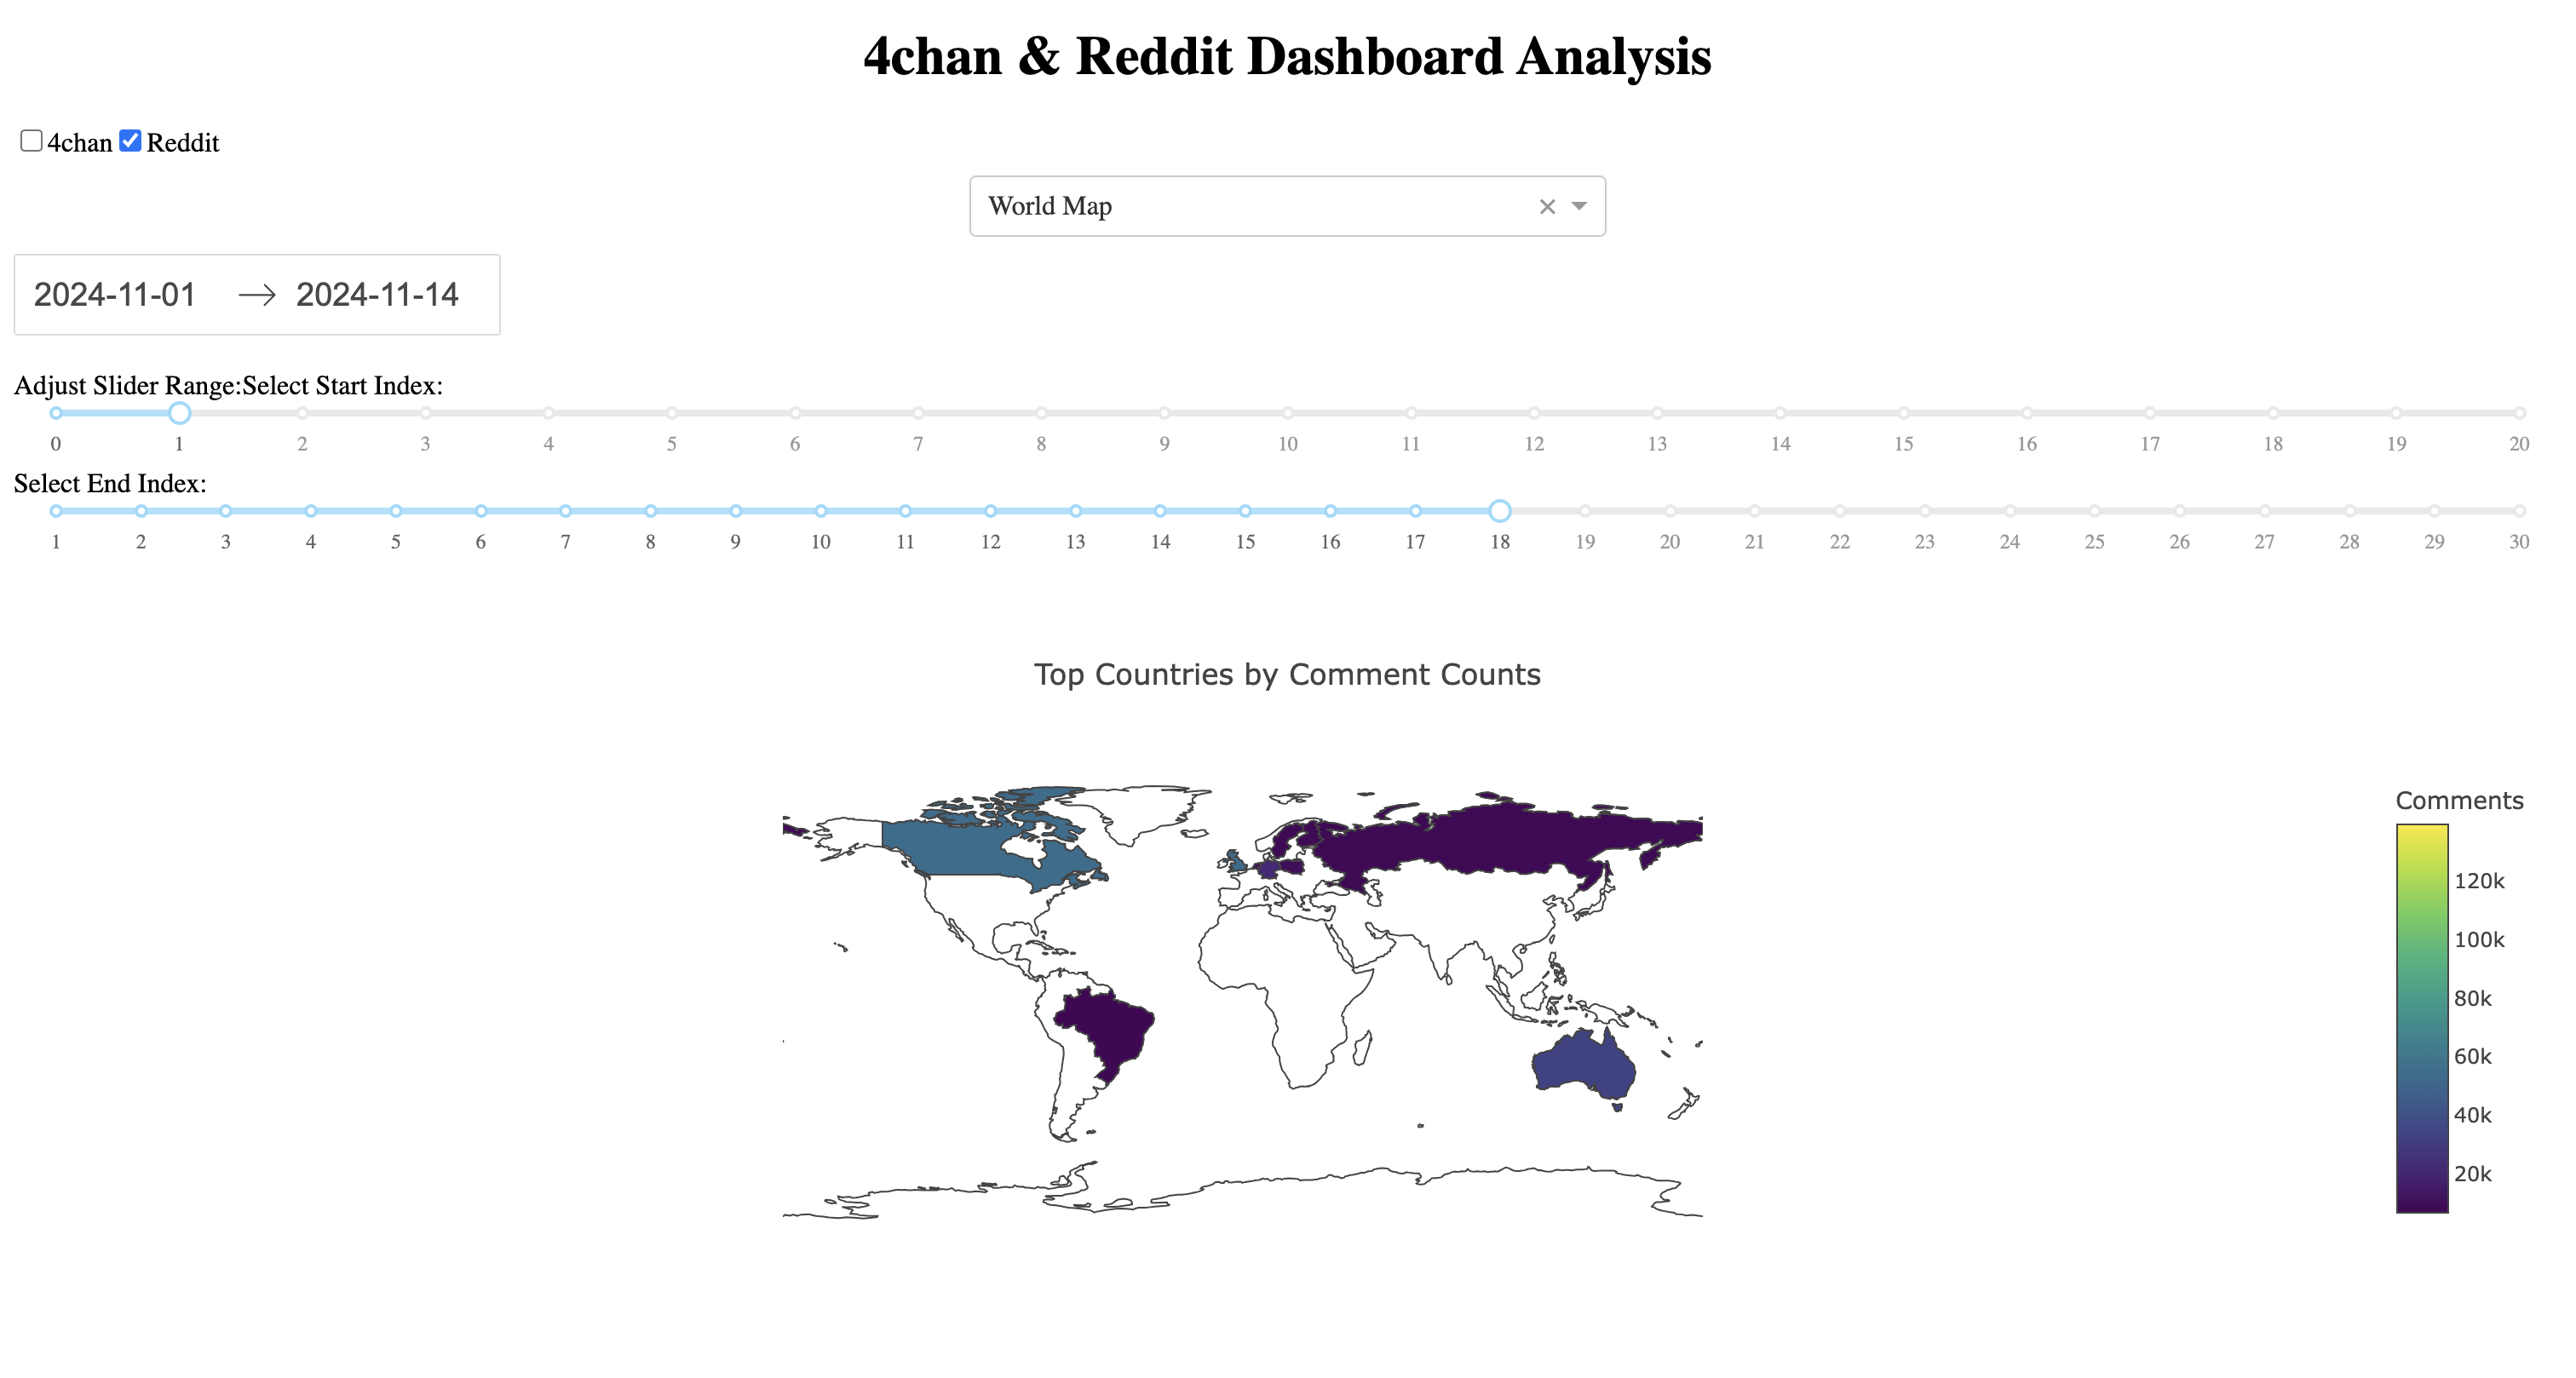
\includegraphics[width=0.5\linewidth]{image-4.png}
        \label{fig:enter-label}
    \end{figure}
    \caption{Country-based comment distribution.}
    \label{fig:country_map}
\end{figure}



\section{Research Questions answered}

\subsection{Research Question}
\subsubsection{How do shifts in sentiment metrics---such as happy, sad, angry, and hopeful---correlate with key events and discussions in U.S. politics?}

{Emotional Spikes and Hierarchy November 6 (U.S. Presidential Election)}
\begin{itemize}
    \item \textbf{Angry} and \textbf{hopeful} emotions dominate:
    \begin{itemize}
        \item \textbf{Angry sentiment} is at its peak, likely driven by contentious election outcomes, allegations of fraud, or dissatisfaction with the process. Anger here may signify frustration among those whose expectations were unmet or fears about future political directions.
        \item \textbf{Hopeful sentiment}, equally prominent, indicates optimism among those who see the election outcome as aligning with their desires or values. This duality highlights the polarized nature of political discussions during elections.
        \item \textbf{Happy sentiment}, though present, is relatively subdued compared to anger and hope. This suggests that celebratory reactions were overshadowed by more intense, conflicting emotions.
        \item \textbf{Sad sentiment} is the lowest, indicating that disappointment or despair is less frequently expressed in comparison to anger or hope. This may reflect a tendency of users to externalize negative emotions through anger rather than introspective sadness.
    \end{itemize}
\end{itemize}

{November 13 (Key Position Announcements)}
\begin{itemize}
    \item \textbf{Angry} and \textbf{hopeful} emotions spike again, continuing the pattern from November 6.
    \begin{itemize}
        \item \textbf{Angry sentiment} remains high, possibly driven by disapproval of announced individuals or policies. It suggests ongoing frustration and debates around the implications of these appointments.
        \item \textbf{Hopeful sentiment}, equally prominent, reflects continued aspirations and expectations for positive changes or outcomes based on the new appointments.
        \item \textbf{Happy} and \textbf{sad} sentiments remain relatively constant, highlighting that the discourse during this event was primarily focused on hope and anger.
    \end{itemize}
\end{itemize}

\begin{figure}
    \centering
    \includegraphics[width=0.5\linewidth]{download (3) (1).png}
    \caption{Sentiment Analysis}
    \label{fig:enter-label}
\end{figure}

\subsubsection{How do temporal patterns in social media activity correlate
with engagement metrics like comments?}
{Emotional Hierarchy Differences}
{Temporal patterns in social media activity, as demonstrated in the comparison between 4chan and Reddit, correlate with engagement metrics like comments by highlighting the influence of platform characteristics and event-driven activity on user interaction.

Key Insights from the Data:
Higher Post Count on 4chan (Doubling Reddit’s Activity):

From November 1 to November 14, 2024, 4chan exhibited consistently higher post counts compared to Reddit, likely driven by its unmoderated and anonymous nature. This environment facilitates uninhibited discussions, particularly around politically charged topics like the 2024 U.S. elections.

Correlation with Engagement Metrics:

On 4chan, the higher post count suggests more immediate and frequent user interactions, which likely translates to increased engagement in terms of comments. The unfiltered nature of discourse encourages rapid responses and ongoing debates.
In contrast, Reddit’s lower post count may correlate with fewer overall comments due to its structured moderation and community guidelines. However, the comments on Reddit posts might reflect deeper, more thoughtful engagement, given the platform's diverse user base and topic range.

Temporal Patterns Reflect Event-Driven Spikes:

The period between November 1 and November 14 encompasses key political events like the U.S. Presidential Election (November 6) and subsequent announcements of key positions (November 13). These events are likely to generate spikes in both post counts and engagement (e.g., comments), with 4chan showing more pronounced activity due to its reactive and real-time nature.

Platform-Specific Dynamics:

On 4chan, the immediacy and intensity of reactions to political events likely drive comment engagement in tandem with post spikes. This aligns with the platform’s culture of rapid, emotionally charged discussions.
Reddit, with its broader topic scope and moderation, might see more consistent but less volatile engagement metrics, as users focus on a variety of discussions beyond the political sphere.}


\begin{figure}
    \centering
    \includegraphics[width=0.5\linewidth]{image (3) (2).png}
    \caption{4Chan vs Reddit comments against time}
    \label{fig:enter-label}
\end{figure}

\subsubsection{How do the tones and volumes of discussions differ between
mentions of different political candidates or parties?}
{The tones and volumes of discussions differ between mentions of political candidates or parties based on geographic trends in engagement, as highlighted by the global distribution of comment activity.

Insights into Tone and Volume:
Volume Differences by Geography:

The choropleth map reveals that countries like Canada contribute the highest number of comments outside the United States, while other countries show varying levels of engagement.
High-comment countries likely have more frequent discussions about U.S. political candidates or parties, potentially reflecting heightened interest in or impact from U.S. policies on these regions.
Tone Variation by Region:

Countries with higher comment activity, such as Canada, may exhibit more diverse tones—ranging from supportive to critical—depending on their political alignment or perceived implications of U.S. political events.
In countries with fewer comments (e.g., those represented in darker brown), discussions might be less polarized or focused, leading to a narrower range of tones.
Candidate or Party Mentions:

Discussions about specific candidates or parties may see differing tones depending on the international perspective. For example:
A candidate perceived as advocating for stronger international ties might elicit more positive discussions in countries with high comment activity.
Conversely, candidates associated with controversial policies could see more critical tones in comments from affected regions.
Engagement Trends by Political Context:

Countries with high engagement levels may reflect broader awareness or emotional investment in U.S. politics, with discussions varying in tone based on the candidate's relevance to their local or global context.
The geographical differentiation underscores that tone and volume are not uniform but influenced by regional interests, cultural factors, and the global implications of U.S. political dynamics.}

\begin{figure}
    \centering
    \includegraphics[width=0.5\linewidth]{newplot (2) (1).png}
    \caption{World map based on number of comments}
    \label{fig:enter-label}
\end{figure}

\section{Conclusion}
This project successfully answered the research questions by implementing analyses that correlated activity and sentiment metrics with social and political contexts. The interactive dashboard facilitates further exploration of these patterns.

\section*{References}
\begin{enumerate}
    \item Social media data processing techniques: \url{https://pandas.pydata.org/}
    \item Plotly visualization library: \url{https://plotly.com/}
    \item Flask framework: \url{https://flask.palletsprojects.com/}
\end{enumerate}

\end{document}
